\documentclass{article}
\usepackage{graphicx}

\begin{document}

\begin{titlepage}
\title{ECS189G Homework 3 Report Problem A}
\author{Goh Chang Kang, Charles 916751838, \\
Yang Minxing 916751773, Chen Jieyi Chloe 999823783}

\date{November 15, 2018}
\maketitle
\end{titlepage}


\section{Problem A}
We used non-negative matrix vectorisation for our prediction. First we loaded the relevant libraries like rectools and updated the functions for trainReco and predict.recoS3 to account for nil user and item ids. 
\begin{verbatim}
trainReco <- function (ratingsIn, rnk = 10, nmf = FALSE) 
{
  require(recosystem)
  hasCovs <- (ncol(ratingsIn) > 3)
  if (hasCovs) {
    covs <- as.matrix(ratingsIn[, -(1:3)])
    lmout <- lm(ratingsIn[, 3] ~ covs)
    minResid <- min(lmout$residuals)
    ratingsIn[, 3] <- lmout$residuals - minResid
  }
  #check for consecutive records.
  #if the max ID is greater than the num of rows, means they are not consecutive
  sMax <- max(ratingsIn[, 1])
  sUnique <- length(unique(ratingsIn[, 1]))
  sOriginal <- ratingsIn[, 1]
  
  dMax <- max(ratingsIn[, 2])
  dUnique <- length(unique(ratingsIn[, 2]))
  dOriginal <- ratingsIn[, 2]
  
  #if they are not consecutive, we use the shrinked ones
  if ((sMax - sUnique) > 0) {
    sortedIdx <- sort(unique(ratingsIn[, 1]))
    sIDTemp <- match(sOriginal, sortedIdx)
    #use the relative position as the new ID, because positions must be consecutive
  } else {
    sIDTemp <- sOriginal
  }
  
  if ((dMax - dUnique) > 0) {
    sortedIdx <- sort(unique(ratingsIn[, 2]))
    dIDTemp <- match(dOriginal, sortedIdx)
  } else {
    dIDTemp <-dOriginal
  }
  
  r <- Reco()
  train_set <- data_memory(sIDTemp, dIDTemp, 
                           ratingsIn[, 3], index1 = TRUE)
  r$train(train_set, opts = list(dim = rnk, nmf = nmf))
  result <- r$output(out_memory(), out_memory())
  attr(result, "hasCovs") <- hasCovs
  if (hasCovs) {
    attr(result, "covCoefs") <- coef(lmout)
    attr(result, "minResid") <- minResid
  }
  class(result) <- "RecoS3"
  #append the attribute for translation purpose
  result$translator <- data.frame(sIDTemp, dIDTemp, sOriginal, dOriginal)
  result
}
predict.RecoS3 <- function (recoObj, testSet) 
{
  p <- recoObj$P
  q <- recoObj$Q
  testSet$pred <- vector(length = nrow(testSet))
  hasCovs <- attr(recoObj, "hasCovs")
  if (hasCovs) {
    covCoefs <- attr(recoObj, "covCoefs")
    minResid <- attr(recoObj, "minResid")
  }
  for (i in 1:nrow(testSet)) {
    j <- testSet[i, 1]
    k <- testSet[i, 2]
    #use the translator to translate to consecutive ID
    originalSIndex <- match(j, recoObj$translator[[3]])
    originalDIndex <- match(k, recoObj$translator[[4]])
    #use the same index to find corresponding shrinked ID
    #the recoObj is still the same
    j <- recoObj$translator[[1]][originalSIndex]
    k <- recoObj$translator[[2]][originalDIndex]
    if (!is.na(j) && !is.na(k) && j <= nrow(p) && k <= nrow(q)) {
      tmp <- 0
      if (hasCovs) 
        tmp <- covCoefs %*% c(1, testSet[i, -(1:3)]) - 
          minResid
      testSet$pred[i] <- p[j, ] %*% q[k, ] + tmp
    }
    else testSet$pred[i] <- NA
  }
  testSet$pred
}
\end{verbatim}

We then split the data into female and male datasets. Due to time and processing constraints, we used a random set of 1,000,000 entries. 

\begin{verbatim}
gender_df = read.table('libimseti/gender.dat', sep = ',')
names(gender_df) = c('User_ID', 'Gender')
rating_df = read.table('libimseti/ratings.dat', sep = ',')
names(rating_df) = c('User_ID', 'Profile_ID', 'Ratings')
# merge the rating_df and gender_df
final_df = merge(rating_df, gender_df, by = 'User_ID')

# get the female and male df
female_df = final_df[which(final_df$Gender == 'F'), ]
male_df = final_df[which(final_df$Gender == 'M'), ]

## We will use predict function to predict the ratings for males and females seprately. 
## preditability = number of correct predictions/ total number of predictions

# Set up male and female data
female_subset = female_df[,1:3]
set.seed(9999)  # so we are all using the same random numbers
testidxs <- sample(1:nrow(female_subset),100000)
female_dataset <- female_subset[testidxs,]
female_testset <- female_dataset[1:10000,]
female_trainset <- female_dataset[10001:100000,]

male_subset = male_df[,1:3]
set.seed(9999)  # so we are all using the same random numbers
testidxs <- sample(1:nrow(male_subset),100000)
male_dataset <- male_subset[testidxs,]
male_testset <- male_dataset[1:10000,]
male_trainset <- male_dataset[10001:100000,]
\end{verbatim}

We decided to use PGEC (Probability of Guessing Exactly Correctly) to test prediction accuracy. These were the two functions we wrote to calculate PGEC vs Rank. Note: Due to the nature of the prediction that gives predictions mostly in decimal rather than whole numbers, we decided to relax the requirement of guessing correctly to < 0.5 difference. This is because when rounding off, one can be at most 0.5 away from a whole number to be rounded off to that number. They would otherwise be 0 if we did not round them to the nearest whole number.

\begin{verbatim}
get_PGEC_accuracy_from_data <- function(trainset, testset, rank) {
  # Extract actual ratings and set master table ratings to NA
  actual_ratings <- testset[3]
  testset[,3] <- NA
  
  # Train model
  trainedModel <- trainReco(trainset, rnk = rank)
  
  # Predict values
  prediction <- predict.RecoS3(trainedModel, testSet = testset)
  
  # Recombined actual values to predicted values and calculate difference
  result <- cbind(prediction, actual_ratings)
  difference <- abs(result['prediction'] - result['Ratings'])
  names(difference) <- c('difference')
  result <- cbind(result, difference)
  print(head(result))
  PGEC = function(df_list) {
    num_rows <- length(which(!is.na(df_list['difference'])))
    accuracy = length(which((df_list['difference'] < 0.5) == TRUE))/num_rows
    return (accuracy)
  }
  }
  pgec_result <- PGEC(result)
}

process_pgec_results <- function(trainset, testset) {
  k_column <- c()
  pgec_column <- c()
  
  # For each rank n, train data set and cross validate, using PGEC error as a benchmark
  lapply(seq(10, 100, 10), function(k) {
    # get PGEC
    pgec <- get_PGEC_accuracy_from_data(trainset, testset, rank = k)
    
    # Append results to result
    k_column <<- c(k_column, k)
    pgec_column <<- c(pgec_column, pgec)
  })
  result <- cbind(k_column, pgec_column)
}
\end{verbatim}

Finally we plot our findings on a line graph.

\begin{verbatim}
female_pgec_results <- process_pgec_results(female_trainset, female_testset)
male_pgec_results <- process_pgec_results(male_trainset, male_testset)
female_pgec_results_df <- as.data.frame(female_pgec_results)
male_pgec_results_df <- as.data.frame(male_pgec_results)

library(ggplot2)
p <- ggplot() +
  # blue plot
  geom_point(data=female_pgec_results_df, aes(x=k_column, y=pgec_column)) + 
  geom_smooth(data=female_pgec_results_df, aes(x=k_column, y=pgec_column), fill="red",
              colour="darkred", size=1) +
  # red plot
  geom_point(data=male_pgec_results_df, aes(x=k_column, y=pgec_column)) + 
  geom_smooth(data=male_pgec_results_df, aes(x=k_column, y=pgec_column), fill="blue",
              colour="darkblue", size=1)
p <- p + ggtitle("Rank vs PGEC for NMF") + xlab("RANK") + ylab("PGEC")
\end{verbatim}

We realised that the results for male were generally more accurate than those for females (blue line represents PGEC for males, and red line represents PGEC for females). We also observed that for both genders, the PGEC increases as the rank increases, which is expected. 

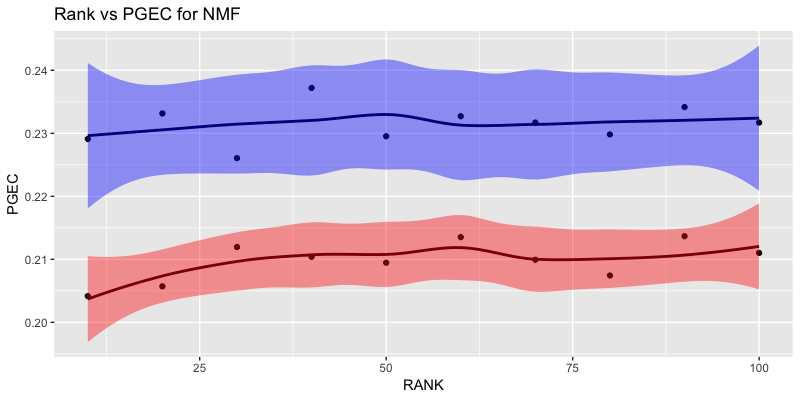
\includegraphics[scale=0.5]{RankvsPGEC.png}

We then decided to test our predictions using MAPE to further verify our findings

\begin{verbatim}
get_MAPE_accuracy_from_data <- function(trainset, testset, rank) {
  # Extract actual ratings and set master table ratings to NA
  actual_ratings <- testset[3]
  testset[,3] <- NA
  
  # Train model
  trainedModel <- trainReco(trainset, rnk = rank)
  
  # Predict values
  prediction <- predict.RecoS3(trainedModel, testSet = testset)
  
  # Recombined actual values to predicted values and calculate difference
  result <- cbind(prediction, actual_ratings)
  
  # MAPE function
  MAPE = function(df_list) {
    inner_sum <- sum(abs(df_list[["Ratings"]] 
    - df_list[["prediction"]])/abs(df_list[['Ratings']]), na.rm=T)
    error = inner_sum/nrow(df_list)
    return (round(error, 3))
  }
  
  mape_result <- MAPE(result)
}

process_mape_results <- function(trainset, testset) {
  k_column <- c()
  mape_column <- c()
  
  # For each rank n, train data set and cross validate, using PGEC error as a benchmark
  lapply(seq(10, 100, 10), function(k) {
    # get PGEC
    mape <- get_MAPE_accuracy_from_data(trainset, testset, rank = k)
    
    # Append results to result
    k_column <<- c(k_column, k)
    mape_column <<- c(mape_column, mape)
  })
  result <- cbind(k_column, mape_column)
}

female_mape_results <- process_mape_results(female_trainset, female_testset)
male_mape_results <- process_mape_results(male_trainset, male_testset)
female_mape_results_df <- as.data.frame(female_mape_results)
male_mape_results_df <- as.data.frame(male_mape_results)

q <- ggplot() +
  # blue plot
  geom_point(data=female_mape_results_df, aes(x=k_column, y=mape_column)) + 
  geom_smooth(data=female_mape_results_df, aes(x=k_column, y=mape_column), fill="red",
              colour="darkred", size=1) +
  # red plot
  geom_point(data=male_mape_results_df, aes(x=k_column, y=mape_column)) + 
  geom_smooth(data=male_mape_results_df, aes(x=k_column, y=mape_column), fill="blue",
              colour="darkblue", size=1)
q <- q + ggtitle("Rank vs MAPE for NMF") + xlab("RANK") + ylab("MAPE")
\end{verbatim}

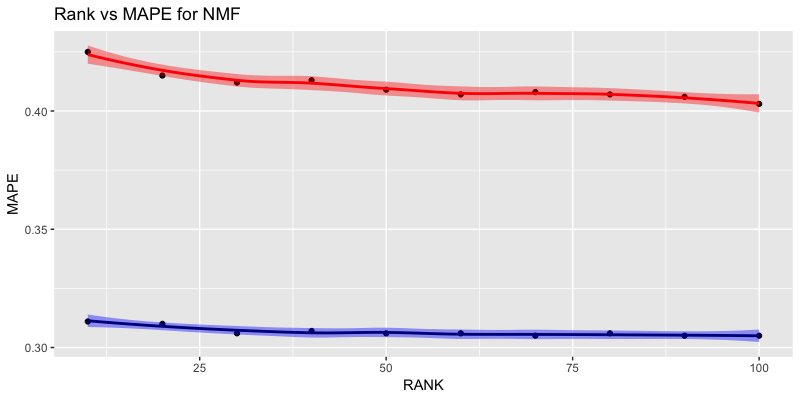
\includegraphics[scale=0.5]{RankvsMAPE.png}

Red line represents MAPE errors for females and blue line represents MAPE errors for males. As expected, the MAPE errors for males were generally lower than those of females, which links to the higher PGEC values for males in our PGEC findings. Therefore, we conclude that males are generally more predictable than females based on our findings.

\end{document}